% Numeric color syntax from pgfplotscolormap.code.tex, applied to a surface.
\documentclass[border=2pt]{standalone}
\usepackage{pgfplots}
\pgfplotsset{compat=1.18,colormap={native}{
  rgb255(0cm)=(12,84,180);rgb255(1cm)=(240,180,32);rgb255(2cm)=(210,40,80)}}
\begin{document}
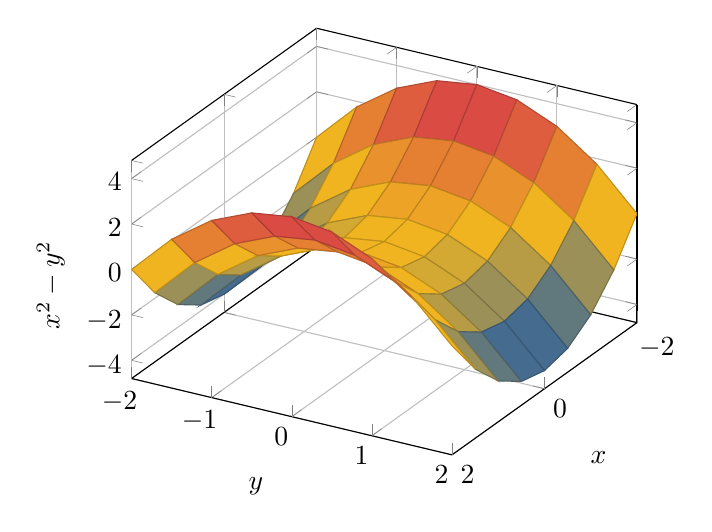
\begin{tikzpicture}
\begin{axis}[width=8cm,height=7cm,view={120}{35},grid=major,
  domain=-2:2,y domain=-2:2,samples=9,samples y=9,
  xlabel=$x$,ylabel=$y$,zlabel=$x^2-y^2$,colormap name=native]
\addplot3[surf] {x^2-y^2};
\end{axis}
\end{tikzpicture}
\end{document}
